
Recall the utterly ridiculous derived amplitude equation for a driven damped oscillator from above:

\begin{equation*}
    A^2 = \frac{f_0^2}{(\omega_o^2 - \omega^2)^2 + 4\beta^2\omega^2}.
\end{equation*}

\noindent Make note that amplitude of the response is proportional to the amplitude of the driving force, $A \propto f_0$. Also note the dependence of $A$ on the frequencies $\omega_o$ (the natural frequency) and $\omega$ (the driving frequency). Specifically, you can see that $A$ is greatest when the two frequencies are almost the same. This is shown is figure \ref{fig:resonance_plot}.

\begin{figure}[h]
    \centering
    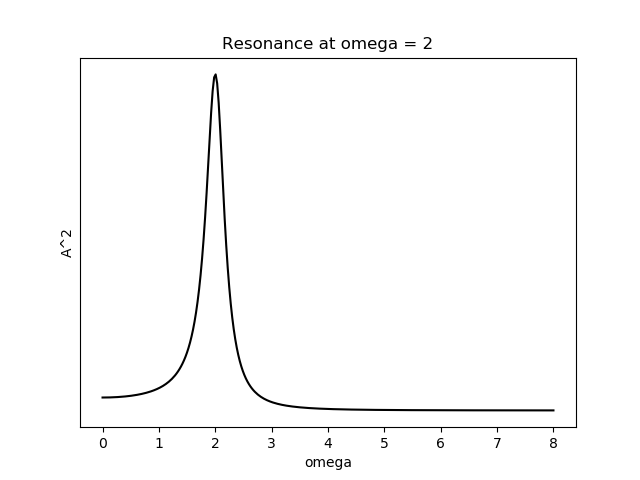
\includegraphics[width=12cm]{Classical_Mechanics/2.13-resonance/A_vs_w_resonance.png}
    \caption{Plotting the amplitude $A^2$ values versus the natural frequency $omega_0$ while holding the driving frequency $\omega$ constant. $\beta = 0.1\omega$ here. Note the peak when $\omega = \omega_o$.}
    \label{fig:resonance_plot}
\end{figure}

This exceptional natural response to the driving frequency is called system {\itshape resonance}.

In order to change the narrowness of the resonance we define something call the {\bfseries full width at half maximum} or {\bfseries FWHM}. This is the interval between the two points where $A^2$ is equal to half its maximum height. These endpoints are $\omega \approx \omega_o \pm \beta$. Thus, FWHM is $\approx 2\beta$.

A quality factor, {\bfseries Q-factor}, is assigned as the ratio between $\omega_o$ and $2\beta$. A large Q-factor indicates a narrow resonance (small $\beta$).
